\documentclass[a4paper,11pt,dvipdfmx]{ujarticle}
% パッケージ
\usepackage{graphicx}
\usepackage{url}
% レイアウト指定を記述したファイルの読み込み
\input{layout}

% タイトルと氏名を変更せよ.
\title{日本におけるデジタル化の状況}
\author{G584312025 鎌田奏太}
\begin{document}
\maketitle 
\section{デジタル競争力ランキング}
国際経営開発研究所(IMD)の調査\cite{imd}によると、日本のデジタル競争力のランキングは図\ref{fig:fok}に示すように、調査対象の64カ国中、総合で28位,技術分野で30位となっている。
\begin{figure}[htbp]
    \centering
    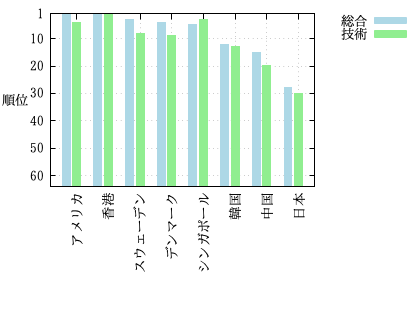
\includegraphics[scale=0.5]{fig41.png}
    \caption{デジタル競争力ランキング(64カ国中)}\label{fig:fok}
\end{figure}
\newpage
\section{ブロードバンドの整備状況}


OECDによるブロードバンド回線の普及に関する調査\cite{oecd}によると,表\ref{fig:dok}に示すように.日本における100人あたりの光ファイバー回線の加入者数は29.0で,韓国,スウェーデン,ノルウェーに続いて第4位になっている.
\begin{table}[htbp]
    \centering
    \caption{光ファイバー回線の加入者数(100人あたり)}\label{fig:dok}
    \begin{tabular}{|c|c|c|}
        \hline
        順位 & 国名 & 加盟者数 \\
        \hline
        1位  &  韓国 & 38.2 \\
        \hline
        2位  &  スウェーデン & 31.9 \\
        \hline
        3位  &  ノルウェー & 29.5 \\
        \hline
        4位  &  日本 & 29.0 \\
        \hline
        5位  &  アイスランド & 28.8 \\
        \hline
        6位  &  スペイン & 27.3 \\
        \hline
        7位  &  ポルトガル & 25.1 \\
        \hline
        8位  &  ニュージーランド & 23.6 \\
        \hline
        9位  &  リトアニア & 22.3 \\
        \hline
        10位  &  フランス & 21.2 \\
        \hline
    \end{tabular}
\end{table}

\section{考察}
\begin{itemize}
    \item 人口の少ない国家が上位10位のほとんどを占めている中で人口の多い日本が上位にいることから環境整備にかなりの力を注いでいると考え力力を注いでいると考えられる。
    \item 教育水準が高いと言われるスウェーデン等の北欧諸国がいることから教育水準も関連していると思われる。
\end{itemize}

% 節見出し: \section{}
% を使う

% 本文(1)
%  参考文献の参照: \cite{}
%  図番号の参照: \ref{}
% を使う
% 文献データベースのキーワードは oecd と imd
% になっている.

% 図の挿入
% \includegraphics{}
% を
% \begin{figure}[htbp]
% \end{figure}
% で囲み
% \caption{}
% で図のタイトルを入れる.
% \label{}
% を使って図番号が参照できるようにする
% また,
% \centering
% で図が中央に来るようにする

% ーーー
% 節見出し(2)

% 本文(2)

% 表の挿入
% \begin{tabular}
% \end{tabular}    
% による表の記述を 
% \begin{table}[htbp]
% \end{table}
% で囲み
% \caption{}
% で表のタイトルを入れる.
% \label{}
% を使って表番号が参照できるようにする
% また,
% \centering
% で表が中央に来るようにする

% ーーー
% 見出し(3)
% 考察
%
% \begin{itemize}
% \end{itemize}
% を使って箇条書きで記述する

% ここに参考文献が入る
%


\bibliographystyle{junsrt}
\bibliography{exercise.bib}

\end{document}